\documentclass[xcolor={dvipsnames,usenames},graphics]{beamer}
%aspectratio=169
%\documentclass[xcolor={dvipsnames},graphics]{beamer}

\usetheme[
progressbar=frametitle,
titleformat=regular,
numbering=counter,
sectionpage=progressbar,
subsectionpage=progressbar,
progressbar=foot, % frametitle,head
block=fill
]{metropolis}

\usepackage{appendixnumberbeamer} %Fixes appendix numbering
%\usepackage{subcaption}
\usepackage[skins,most]{tcolorbox} %Used in header
\usepackage{xspace}
\usepackage{graphicx}
\usepackage[usenames,dvipsnames]{xcolor}
\usepackage{listings}% To typeset programming code
\lstset{
  basicstyle=\ttfamily,
  mathescape
}


% https://tex.stackexchange.com/questions/369758/how-can-i-edit-the-progress-bar-in-beamer-from-a-template-theme/369852#369852
\makeatletter
\setlength{\metropolis@progressinheadfoot@linewidth}{2pt}
\makeatother

\definecolor{PUIblue}{HTML}{265077}
\definecolor{PUIlightblue}{HTML}{657C9D}
\definecolor{PUIorange}{HTML}{F0AD4E}
\definecolor{PUIgray}{HTML}{F1F0EC}

\setbeamercolor{frametitle}{parent=structure,bg=PUIblue,fg=white}
\setbeamercolor{background canvas}{bg=white}
\setbeamercolor{block title example}{fg=white,bg=PUIblue}
\setbeamercolor{block body example}{fg=white,bg=PUIlightblue}

\setbeamerfont{frametitle}{size=\small}
\setbeamerfont{bibliography item}{size=\scriptsize}
\setbeamerfont{bibliography entry author}{size=\scriptsize}
\setbeamerfont{bibliography entry title}{size=\scriptsize}
\setbeamerfont{bibliography entry location}{size=\scriptsize}
\setbeamerfont{bibliography entry note}{size=\scriptsize}
\setbeamerfont{section in toc}{family=\bfseries}

% new caption format
\setlength\abovecaptionskip{-6pt}
\setlength\belowcaptionskip{-5pt}
\setbeamerfont{caption}{size=\tiny}
\setbeamertemplate{caption}{\raggedright \scalebox{.8}{\textcolor{Gray}{Source: \insertcaption}\par}}
\newcommand{\rotatedcaption}[1]{\rotatebox{90}{\tiny \scalebox{0.8}{\textcolor{Gray}{Source: {#1}}}}}
%\newcommand{\rotatedcaption}[2]{\rotatebox{90}{\tiny \scalebox{0.8}{\parbox{{#2}}{\textcolor{Gray}{Source: {#1}}}}}}

\setbeamertemplate{toc subsection itemsep}{\vspace{2ex}}


\settowidth{\leftmargini}{\usebeamertemplate{itemize item}}
\addtolength{\leftmargini}{\labelsep}
%\setbeamersize{text margin left=1cm,text margin right=1cm} 

% customize citations
\usepackage{natbib}
\renewcommand{\bibsection}{}
\setcitestyle{authoryear,round,open={[},close={]}}

% show small symbol next to urls
\usepackage{fontawesome}
\usepackage{hyperref}
\let\orighref\href
\renewcommand{\href}[2]{\orighref{#1}{#2\,~{\tiny \faExternalLink}}}

% https://tex.stackexchange.com/questions/225736/latex-beamer-define-itemsep-globally
\usepackage{xpatch}
\makeatletter
\newcommand{\my@beamer@setsep}{%
\ifnum\@itemdepth=1\relax
     \setlength\itemsep{\my@beamer@itemsepi}% separation for first level
   \else
     \ifnum\@itemdepth=2\relax
       \setlength\itemsep{\my@beamer@itemsepii}% separation for second level
       \setlength\topsep{\my@beamer@itemsepii}% separation for second level
     \else
       \ifnum\@itemdepth=3\relax
         \setlength\itemsep{\my@beamer@itemsepiii}% separation for third level
         \setlength\topsep{\my@beamer@itemsepiii}% separation for second level
   \fi\fi\fi}
\newlength{\my@beamer@itemsepi}\setlength{\my@beamer@itemsepi}{2ex}
\newlength{\my@beamer@itemsepii}\setlength{\my@beamer@itemsepii}{1ex}
\newlength{\my@beamer@itemsepiii}\setlength{\my@beamer@itemsepiii}{1ex}
\newcommand\setlistsep[3]{%
    \setlength{\my@beamer@itemsepi}{#1}%
    \setlength{\my@beamer@itemsepii}{#2}%
    \setlength{\my@beamer@itemsepiii}{#3}%
}
\xpatchcmd{\itemize}
  {\def\makelabel}
  {\my@beamer@setsep\def\makelabel}
 {}
 {}

\xpatchcmd{\beamer@enum@}
  {\def\makelabel}
  {\my@beamer@setsep\def\makelabel}
 {}
 {}
\makeatother

% redefine columns environment
% https://tex.stackexchange.com/questions/204022/make-onlytextwidth-default-width-of-columns
\makeatletter
\long\def\beamer@newenvnoopt#1#2#3#4{%
    \expandafter\renewcommand\expandafter<\expandafter>\csname#1\endcsname[#2]{#3}%<- here
    \expandafter\long\expandafter\def\csname end#1\endcsname{#4}%
}
\long\def\beamer@newenvopt#1#2[#3]#4#5{%
    \expandafter\renewcommand\expandafter<\expandafter>\csname#1\endcsname[#2][#3]{#4}%<- here
    \expandafter\long\expandafter\def\csname end#1\endcsname{#5}%
}

\renewenvironment<>{columns}[1][]{%
    \begin{actionenv}#2%
        \def\beamer@colentrycode{%
            \hbox to\textwidth\bgroup%
            \leavevmode%
            \hskip-\beamer@leftmargin%
            \nobreak%
            \beamer@tempdim=\textwidth%
            \advance\beamer@tempdim by\beamer@leftmargin%
            \advance\beamer@tempdim by\beamer@rightmargin%
            \hbox to\beamer@tempdim\bgroup%
            \hbox{}\hfill\ignorespaces}%
        \def\beamer@colexitcode{\egroup%
            \nobreak%
            \hskip-\beamer@rightmargin\egroup}%
        \ifbeamer@centered\setkeys{beamer@col}{c}\else\setkeys{beamer@col}{t}\fi%
        \setkeys{beamer@col}{#1, onlytextwidth}% added "onlytextwidth"
        \par%
        \beamer@colentrycode%
        \def\beamer@colclose{}\ignorespaces}%
    {\beamer@colclose\def\beamer@colclose{}\beamer@colexitcode\end{actionenv}}%
\makeatother

% TIKZ defaults
\tikzset{basic/.style={draw,fill=PUIblue!20,text width=1em,text badly centered}}
\tikzset{input/.style={basic,circle}}
\tikzset{weights/.style={basic,rectangle}}
\tikzset{functions/.style={basic,circle,fill=PUIlightblue!10}}

% change title page
\setbeamertemplate{title page}{
\begin{minipage}[b][\paperheight]{\textwidth}
    \ifx\inserttitlegraphic\@empty\else\usebeamertemplate*{title graphic}\fi
    \vfill%
    \ifx\inserttitle\@empty\else\usebeamertemplate*{title}\fi
    \ifx\insertsubtitle\@empty\else\usebeamertemplate*{subtitle}\fi
    \usebeamertemplate*{title separator}
    \ifx\beamer@shortauthor\@empty\else\usebeamertemplate*{author}\fi
    \ifx\insertdate\@empty\else\usebeamertemplate*{date}\fi
    \ifx\insertinstitute\@empty\else\usebeamertemplate*{institute}\fi
%    \vfill
    \vspace*{1cm}
%    \vspace*{1mm}
\end{minipage}
}

%%%%%%%%%%%%%ENTER TITLE AND AUTHOR HERE%%%%%%%%%%%%%%%%%%
\title{Gaze-based Transformer for Improving Action Recognition in Egocentric Videos}
\subtitle{Master Thesis}
\date{\today}
%\date{\lectureyear}
\author{Mengze Lu}
\institute{Perceptual User Interfaces Group, University of Stuttgart\\[0.1cm] \href{https://www.perceptualui.org/}{www.perceptualui.org}}
\titlegraphic{
\hfill

\includegraphics[height=0.6cm]{assets/PUI_color3.png}
\hspace{0.4cm}
%\includegraphics[height=0.6cm]{ellis_logo.png}
%\hspace{0.4cm}

\includegraphics[height=0.7cm]{assets/USTUTT_logo.pdf}
}

% https://tex.stackexchange.com/questions/6185/absolute-positioning-in-beamer
\logo{
\begin{tikzpicture}[overlay,remember picture]
\node[anchor=south west,yshift=0.2cm,xshift=0.2cm] at (current page.south west){
    
\includegraphics[height=0.7cm]{assets/PUI.png}
};
\end{tikzpicture}
}

\begin{document}

\maketitle

\AtBeginSection[]
{
\begin{frame}
  \frametitle{Table of Contents}
  \tableofcontents[currentsection]
\end{frame}
}

% ==============================================
\section[Introduction]{Introduction}

%\subsection{Action Recognition}
\begin{frame}{Action Recognition}
	\begin{figure}
		\begin{minipage}{0.45\textwidth}
			\textbf{Task:}
			\begin{itemize}
				\item Identify and categorize human actions into predefined classes.
%				\item \textbf{Goal:} Accurately classify the actions into predefined classes.
			\end{itemize}
		\end{minipage}
		\hfill
		\begin{minipage}{0.5\textwidth}
			\centering
			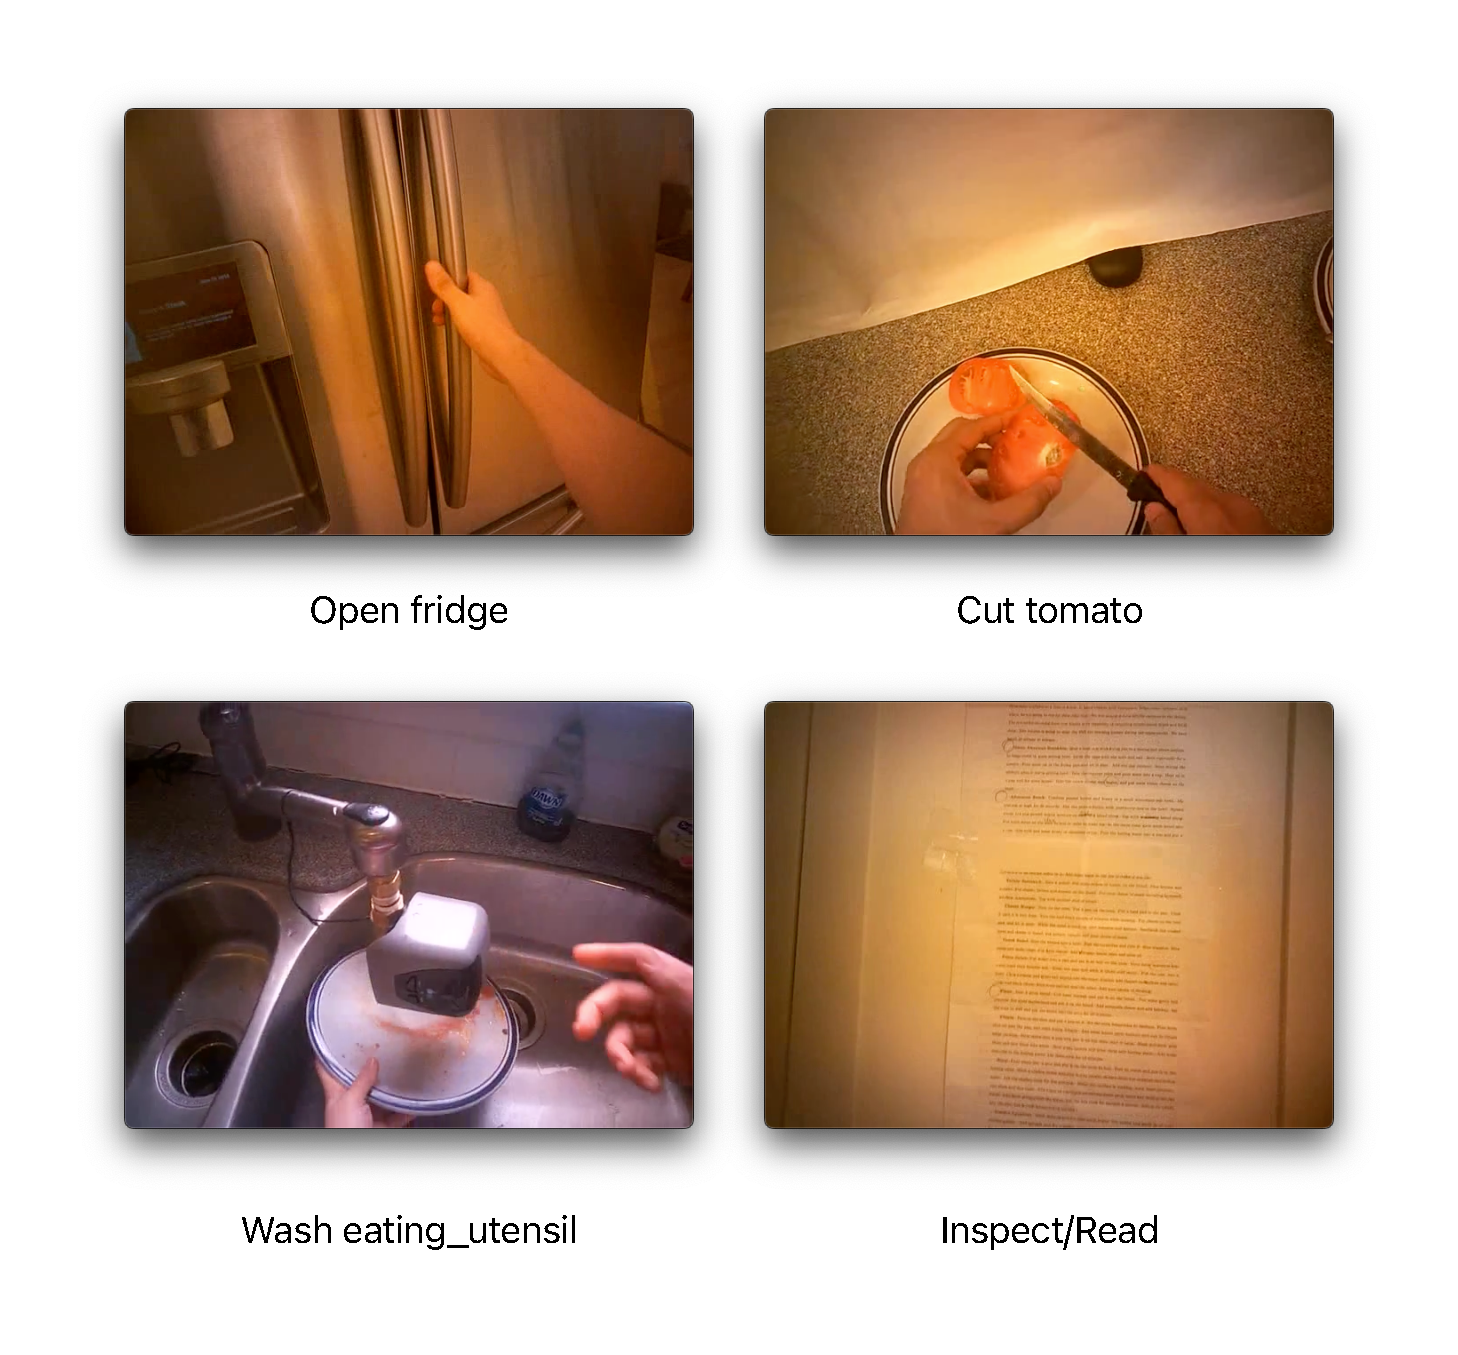
\includegraphics[width=1\linewidth]{assets/action_recognition} 
			\caption{Videos with action labels}
			\label{fig:Action Recognition}
		\end{minipage}
	\end{figure}
\end{frame}

%\subsection{Egocentric Video}
\begin{frame}[fragile]{Egocentric Video}
	\begin{figure}
		\begin{minipage}{0.8\textwidth}
			\centering
			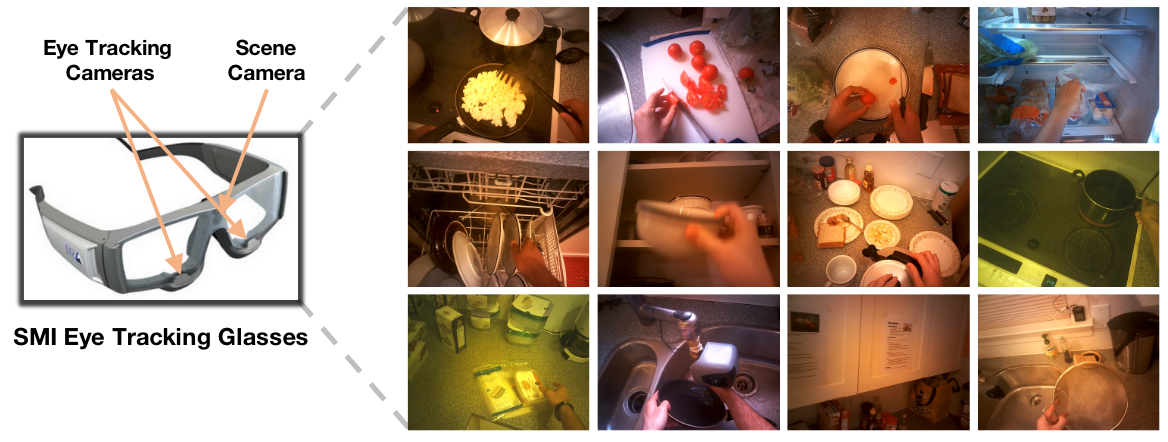
\includegraphics[width=1\linewidth]{assets/egocentric_video} 
			\caption{\cite{li2020eye} Eye tracking glasses used in video recording.}
			\label{fig:Egocentric Video}
		\end{minipage}
		\vfill % Optional: add some space between the two minipages
		\begin{minipage}{0.9\textwidth}
			\textbf{Key Features:}
			\begin{itemize}
				\item First-person view (FPV)
				\item Hand and object interactions
				\item Large scene changes and diverse backgrounds
				% \item Temporal information 
			\end{itemize}
		\end{minipage}
	\end{figure}
\end{frame}

%\subsection[Significance of Gaze in Action Recognition]{Significance of Gaze in Action Recognition}
\begin{frame}[fragile]{Significance of Gaze in Action Recognition} 
	Gaze information:
	\begin{itemize}
		\item Crucial for understanding human intention
		\item Closely linked to object-oriented actions	
	\end{itemize}
	Benefits of adding Gaze Information:
	\begin{itemize}
		\item Enhances the precision of action recognition
	\end{itemize}
\end{frame}
\begin{frame}{The Goal of this Thesis}
	\textbf{Objective:}
	Improve the accuracy of transformers for action recognition by integrating gaze data.
\end{frame}

\section[Related Works]{Related Works}

\subsection[Video Swin Transformer]{Video Swin Transformer}
%\begin{frame}[fragile]{Transformers in Video Recognition}
%	\textbf{Historical Context:} \\
%	Previously, CNNs were the dominant model for action recognition
%	
%	%However, a modeling shift is currently underway on backbone architectures for image classification, from Convolutional Neural Networks (CNNs) to Transformers
%	
%	\textbf{Recent Developments:}
%	\begin{itemize}
%		\item \cite{dosovitskiy2021image} introduced the Vision Transformer
%		\item \cite{liu2021video} proposed the Video Swin Transformer
%		\item \cite{pan2023egovit} developed the Pyramid Video Transformer (EgoViT)
%	\end{itemize}
%\end{frame}


\begin{frame}[fragile]{Video Swin Transformer}
	\begin{figure}
		\centering
		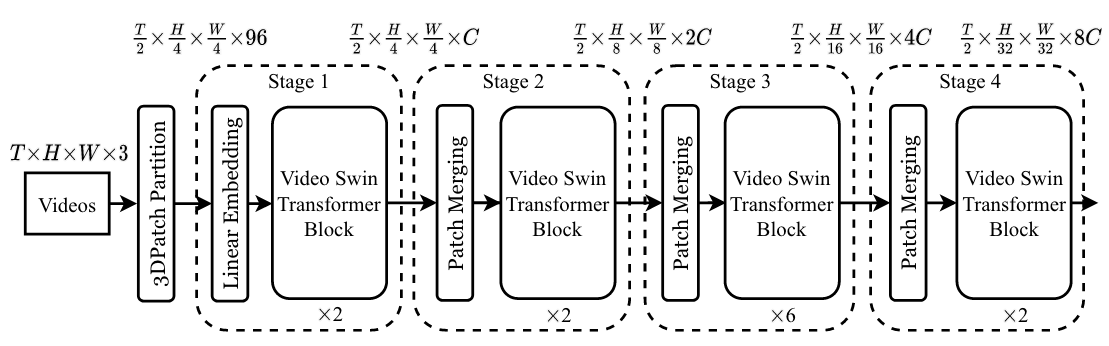
\includegraphics[width=\linewidth]{assets/SwinT}
		\caption{Overview of the Video Swin Transformer Architecture. \cite{liu2021video}}
		\label{fig:SwinT}
	\end{figure}	
	\begin{minipage}{\textwidth}
		\begin{itemize}
			\item Processes inputs through a series of Swin Transformer blocks
			\item Utilizes 3D Shifted Window Self-Attention to handle local relationships %: handel spatial and temperol relationships in video data.
			\item Serves as the backbone in the proposed model.
		\end{itemize}
	\end{minipage}
\end{frame}


%\begin{frame}[fragile]{Transformers in Video Recognition}
%	Advantages of Transformers in Video Recognition:
%	
%	\begin{itemize} % \begin{itemize} to have numbered lists
%			\item Effective for comprehensive image classification.
%			\item Archive success in video recognition tasks.
%			\item Potentially reduce the computational costs.
%		\end{itemize}
%	\end{frame}

\subsection[Vision Transformer EgoViT]{Vision Transformer EgoViT}
\begin{frame}{Vision Transformer EgoViT}
	\begin{figure}
		\begin{minipage}{0.8\textwidth}
			\centering
			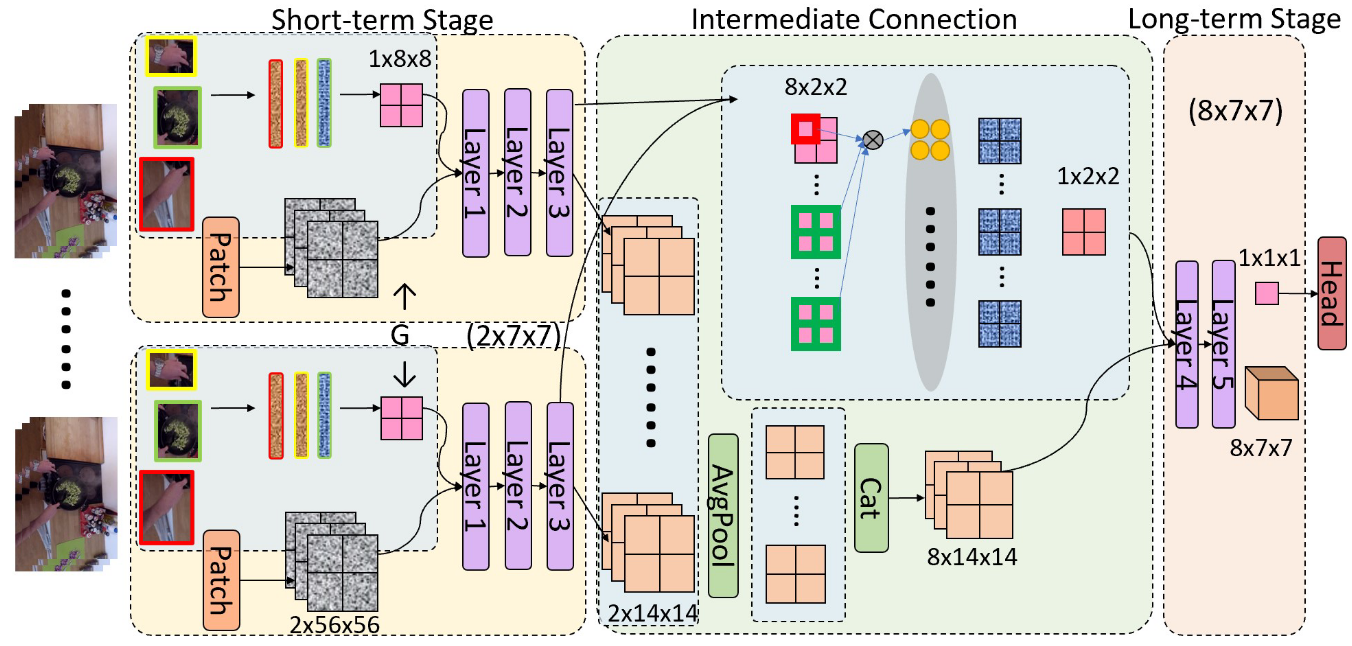
\includegraphics[width=0.9\linewidth]{assets/EgoViT} 
			\caption{\cite{pan2023egovit} The structure of EgoViT.}
			\label{fig:EgoViT}
		\end{minipage}
		\vfill % Optional: add some space between the two minipages
		\begin{minipage}{1\textwidth}
%			Contribution of EgoViT:
%			%\begin{itemize}
%			%    \item Designed for egocentric data
%			%    \item Seamlessly integrate with different video transformers
%			%\end{itemize}
%			\begin{itemize}
%				\item Take Hand-Object features into account
%				\item Dynamic class token (DCT): Focus on the informative parts
%				\item Pyramid Architecture with Dynamic Merging (PADM): Properly processing large movements
%			\end{itemize}
			\textbf{Features:}
			\begin{itemize}
			   \item Designed for egocentric video.
			   \item Seamlessly integrates with different vision transformers
			\end{itemize}
		\end{minipage}
	\end{figure}
\end{frame}

\begin{frame}{State-of-the-Art Vision Transformer EgoViT}
	\textbf{Contribution of EgoViT:}
	%\begin{itemize}
	%    \item Designed for egocentric data
	%    \item Seamlessly integrate with different video transformers
	%\end{itemize}
	\begin{itemize}
		\item Incorporates hand-object interaction features.
		\item Dynamic class token (DCT): Focuses on the informative parts.
		\item Pyramid Architecture with Dynamic Merging (PADM): Effectively processes large movements.
	\end{itemize}
\end{frame}

% \subsection[Joint model of FPV gaze and actions]{Joint model of FPV gaze and actions}
% %\begin{frame}{Studies on Gaze Information}
% %	\begin{itemize}
% %		\item \cite{huang2018predicting} developed a CNN model specifically for gaze estimation.
% %		\item \cite{lai2022eye} introduced a transformer-based model for egocentric gaze estimation.
% %	\end{itemize}
% %\end{frame}
% \begin{frame}{Joint model of FPV gaze and actions}
% 	\begin{figure}
% 		\centering
% 		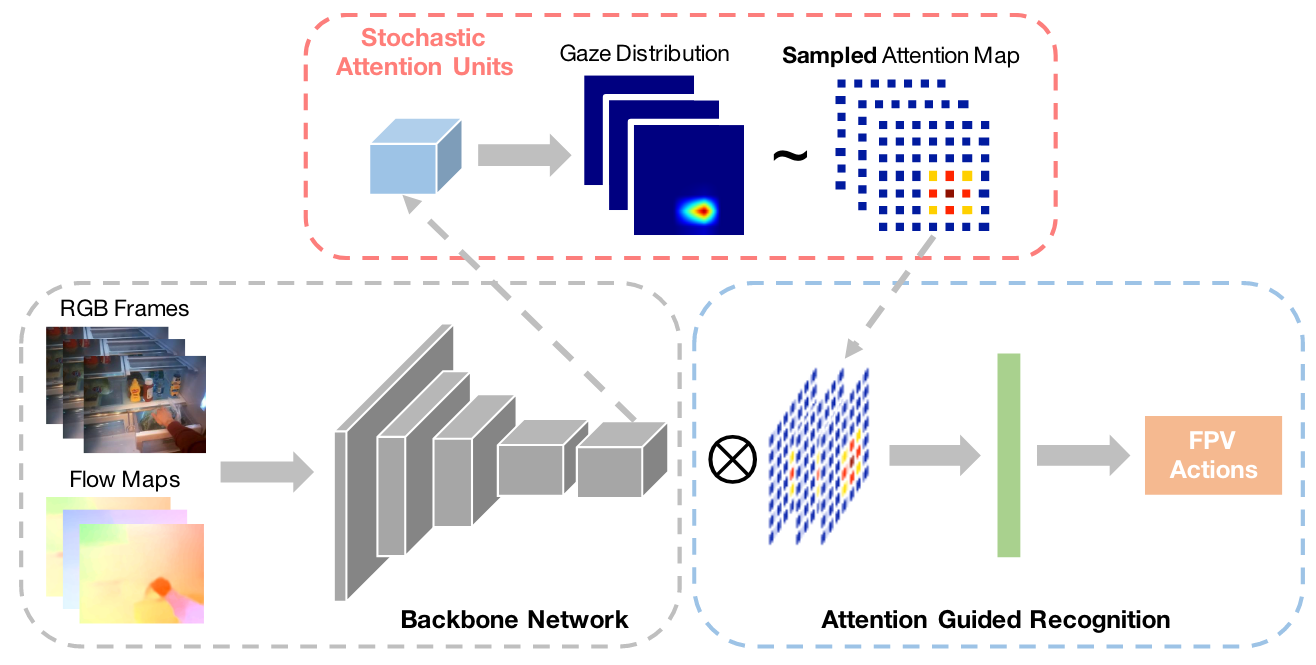
\includegraphics[width=0.8\linewidth]{assets/joint_gaze_action}
% 		\caption{Overview of joint model of FPV gaze and actions. \cite{li2020eye}}
% 		\label{fig:jointgazeaction}
% 	\end{figure}
% 	\begin{itemize}
% 		\item The model is highly relevant to Conditional Variational Autoencoder
% 		\item A distribution of gaze is defined in the middle layers

% 	\end{itemize}
% \end{frame}



\section[Gaze Enhanced EgoViT]{Gaze Enhanced EgoViT}

\subsection[Gaze Enhanced EgoViT Structure]{Gaze Enhanced EgoViT Structure}

\begin{frame}{Gaze Enhanced EgoViT Structure}
	\begin{figure}
		\begin{minipage}[t]{1\textwidth}
			\centering
			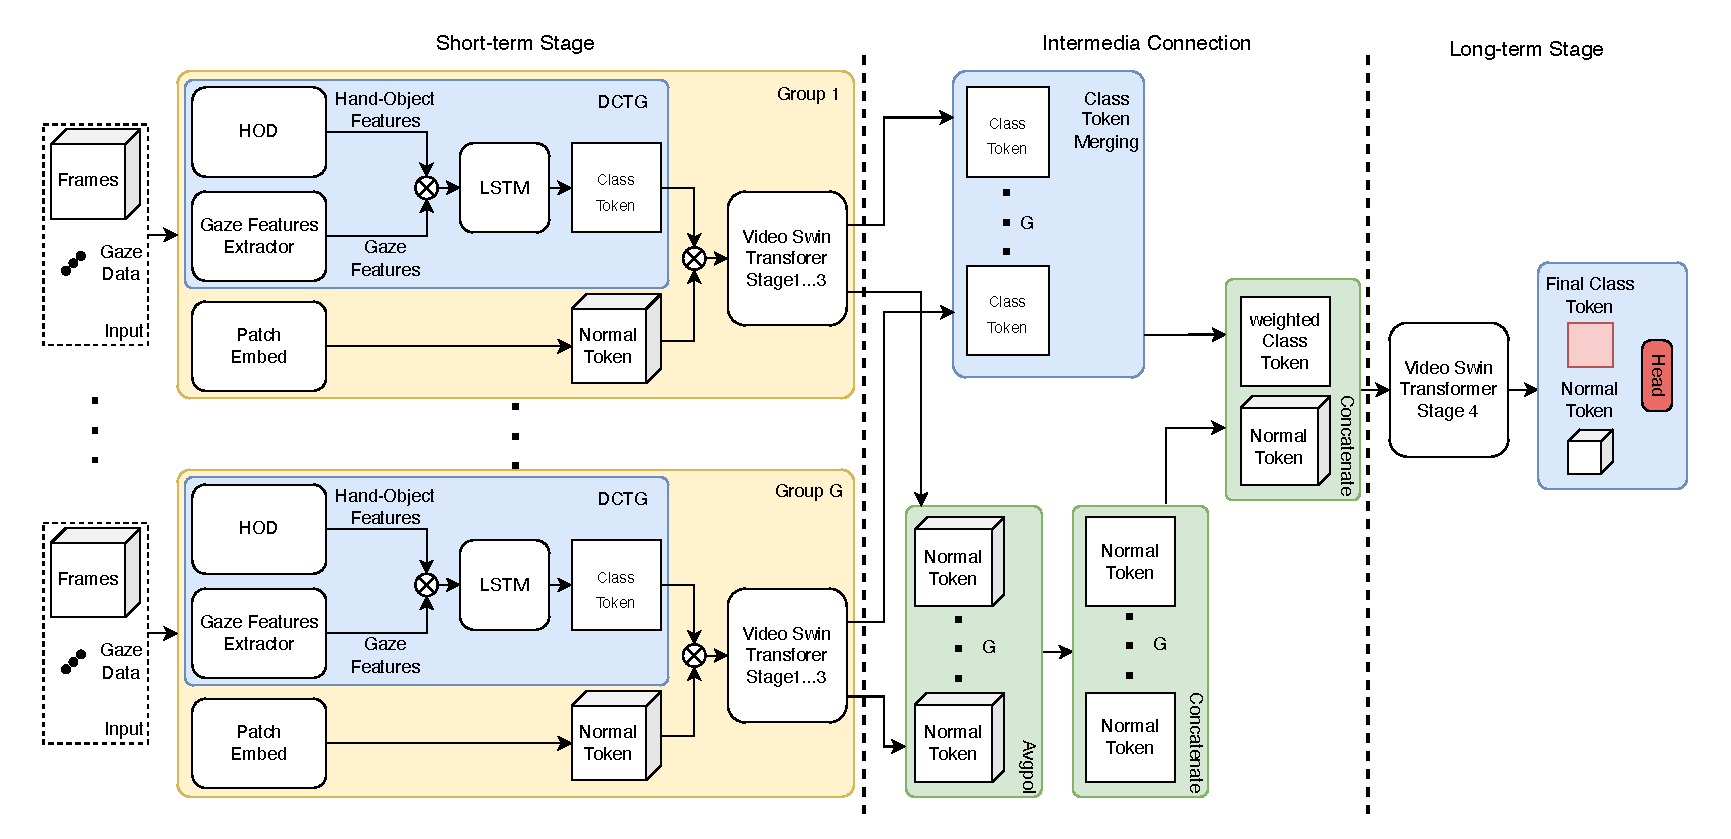
\includegraphics[scale=0.4]{assets/structure.pdf}
			\caption{The Structure of Gaze Enhanced EgoViT}
			\label{fig:Structure of Model}
		\end{minipage}
		\vfill
		\begin{minipage}[t]{0.9\textwidth}
			\begin{itemize}
				\item Architecture: Based on EgoViT
				\item DCTG extended with gaze features extraction module
%				\item Class Token is generated from Hand-Gaze-Object features
			\end{itemize}
		\end{minipage}
	\end{figure}
\end{frame}

\subsection[Key Components]{Key Components}

\begin{frame}{Gaze Enhanced DCTG}
	\begin{minipage}[t]{1\textwidth}
		\begin{figure}
			\centering
			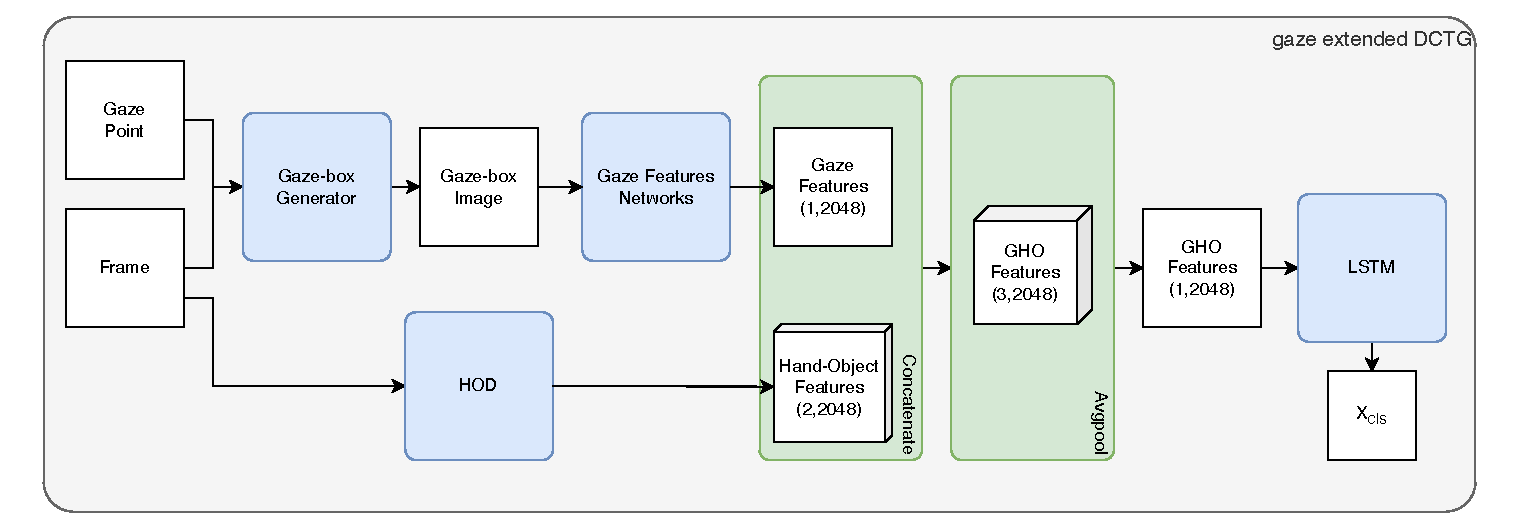
\includegraphics[width=\linewidth]{assets/dctg.pdf}
			\caption{Illustration of the Dynamic Class Token Generator with Gaze Information.}
			\label{fig:enhanceddctg}
		\end{figure}
	\end{minipage} \vfill
	\begin{minipage}[t]{1\textwidth}
		\begin{itemize}
			% \item Use a gaze-box approach for more robust feature extraction.
			\item Gaze features (G) and Hand-Object features (HO) are fused to form GHO features.
			\item Employs an LSTM to generate the class token, enhancing temporal coherence.
		\end{itemize}
	\end{minipage}
\end{frame}
\begin{frame}{Gaze Features Extraction}
	\begin{figure}
		\centering
		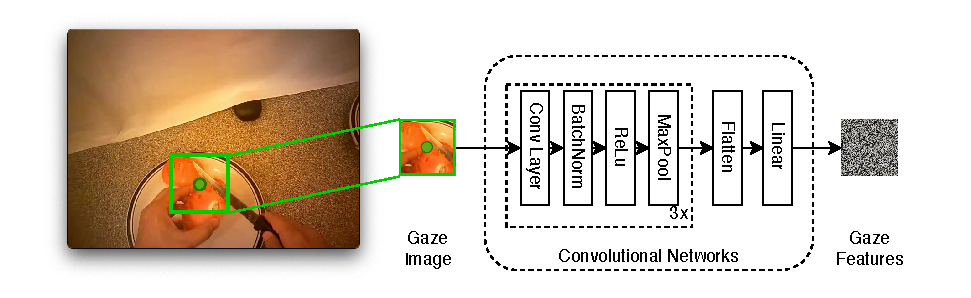
\includegraphics[width=\linewidth]{assets/g_net.pdf}
		\caption{Illustration of the Gaze Features Extraction.}
		\label{fig:shortterm}
	\end{figure}
	\vspace{5mm}
	\textbf{Process:} \\
	Gaze point $\rightarrow$ Gaze-box image $\rightarrow$ Convolutional Networks $\rightarrow$ Gaze features
	% Gaze point $\rightarrow$ gaze-box image $\rightarrow$ Conv Networks $\rightarrow$ gaze features
\end{frame}
%\begin{frame}{Video Swin Transformer Backbone}
%	\begin{figure}
%		\centering
%		\begin{minipage}{0.59\textwidth}
%			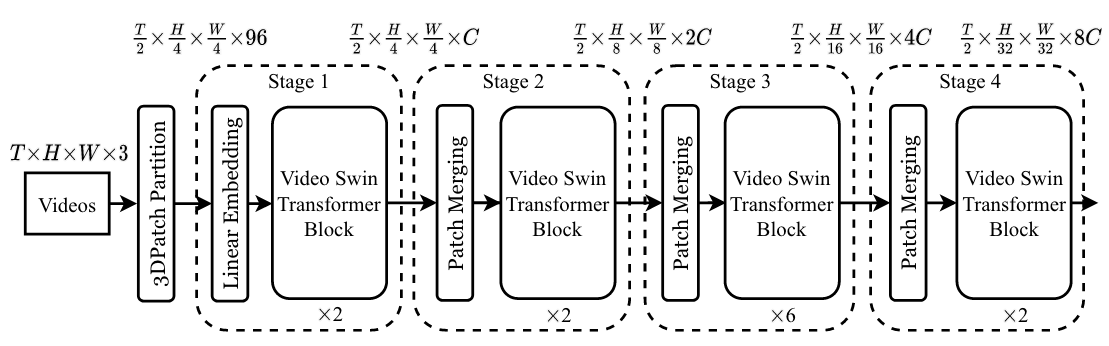
\includegraphics[width=\linewidth]{assets/SwinT}
%			\caption{Overview of the Video Swin Transformer Architecture. \cite{liu2021video}}
%			\label{fig:SwinT}
%		\end{minipage}
%		\hfill
%		\begin{minipage}{0.39\textwidth}
%			\centering
%			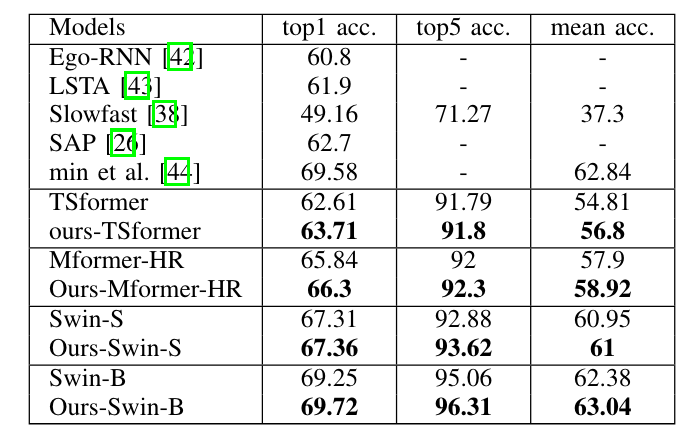
\includegraphics[width=\linewidth]{assets/table_acc}
%			\caption{EAR results of various transformers on the EGTEA GAZE+.\cite{pan2023egovit}}
%			\label{fig:tableacc}
%		\end{minipage}
%	\end{figure}
%	\begin{minipage}{\textwidth}
%		\begin{itemize}
%			\item 3D Shifted Window Self-Attention: handel spatial and temperol relationships in video data.
%			\item Achive best performance with EgoviT.
%%			\item Use Video Swin Transformer as backbone
%		\end{itemize}
%	\end{minipage}
%\end{frame}

\begin{frame}{Dynamic Merging Module}
	\begin{minipage}{\textwidth}
		\begin{figure}
			\centering
			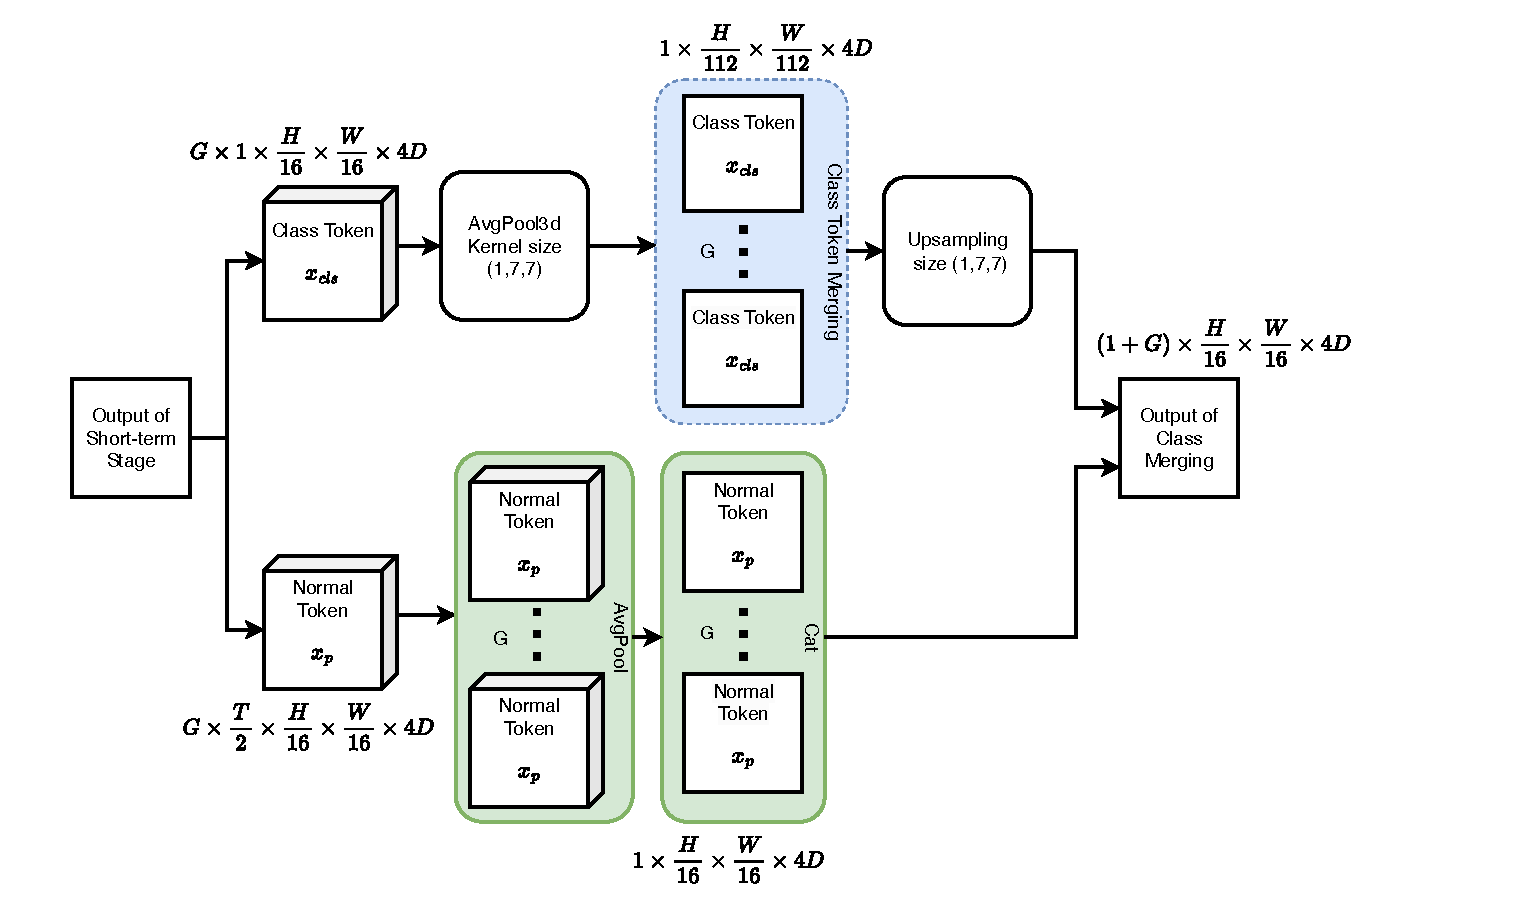
\includegraphics[width=0.8\linewidth]{assets/dm.pdf}
			\caption{Illustration of the Dynamic Merging Module.}
			\label{fig:xclsmerg}
		\end{figure}
	\end{minipage}
	\vfill
	\begin{minipage}{\textwidth}
		\begin{itemize}
			\item The class token and normal token are merged separately.
			\item Input $\rightarrow$ G-$x_{cls}$, G-$x_p$ $\rightarrow$ Weighted $x_{cls}$, $x_p$ $\rightarrow$ Concat. output
		\end{itemize}
	\end{minipage}
% 	\begin{minipage}{\textwidth}
% 		\begin{itemize}
% 			% \item Class token and normal token merged seperately
% %			\item G parallel layers in Short-term stage
% %			\item The weighted class token is calculated from G class tokens.
% 		\end{itemize}
	% \end{minipage}
\end{frame}

\section[Experiments]{Experiments and Results}
\begin{frame}{Dataset}
	\begin{figure}
		\begin{minipage}{0.55\textwidth}
			\textbf{EGTEA Gaze+}:A large-scale dataset for FPV actions and gaze analysis
			\begin{itemize}
				% \item 10321 trimmed action videos (640x480 at 24Fps)
				\item Gaze tracking data available at 30Fps
				\item Frame-level action annotations
			\end{itemize}
		\end{minipage}%
		\hfill % Optional: add some space between the two minipages
		\begin{minipage}{0.45\textwidth}
			\centering
			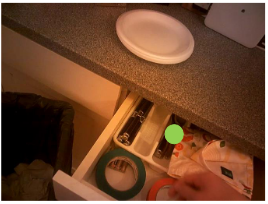
\includegraphics[width=0.9\linewidth]{assets/gaze_plus} 
			\caption{\cite{li2020eye} A frame from the dataset showing gaze point. }
			\label{fig:dataset}
		\end{minipage}
	\end{figure}	
\end{frame}

\begin{frame}{Dataset}
	\begin{itemize}
		\item Gaze-Hand-Object (GHO) features are preprocessed offline.
		% \item The training dataset consists of frames, GHO-features and action labels.
		\item Each video is sampled at an average of 32 frames.
		\item Dataset structure: \\
			(Frames[32,3,224,224], GHO-Features[32,3,2048], Label[1]) 
		% \item GHO-features have a shape of [32, 5, 2048] % which includes 1 gaze, 2 hand and 2 object features per frame.
	\end{itemize}
\end{frame}

% \begin{frame}{Dataset Modifications}
% 	\begin{figure}
% 		\begin{minipage}{0.45\textwidth}
% 			% \textbf{EGTEA Gaze+}: a large-scale dataset for FPV actions and gaze
% 			\centering
% 			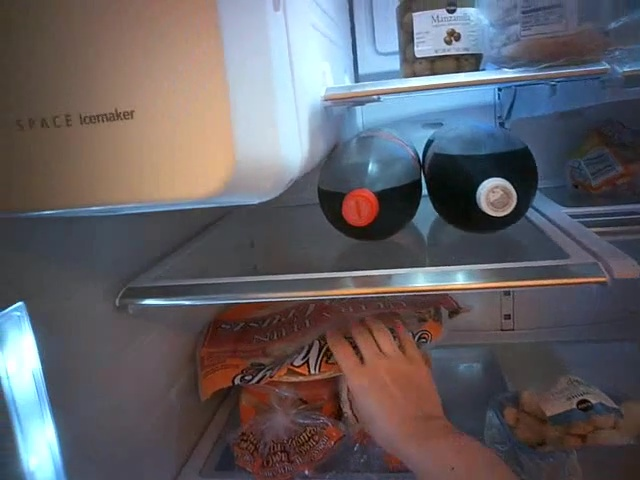
\includegraphics[width=0.6\linewidth]{assets/one_hand}
% 			\caption{A frame contants one hand and one object}
% 			\label{fig:two_hand}
% 			\vspace{6mm}
% 			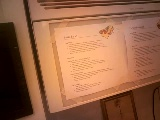
\includegraphics[width=0.6\linewidth]{assets/only_gaze}
% 			\caption{A frame only including gaze info.}
% 			\label{fig:only_gaze}
% 		\end{minipage}%
% 		\hfill % Optional: add some space between the two minipages
% 		\begin{minipage}{0.5\textwidth}
% 			\begin{itemize}
% 				\item Not all frames contain two hands.
% 				\item Some video actions include only gaze information
% 				\item A few videos (about 1\%) lack gaze data
% 			\end{itemize}
% 		\end{minipage}
% 	\end{figure}
% \end{frame}

\begin{frame}{Training the Original EgoViT}
    \begin{minipage}{0.5\textwidth}
        % \centering
        \begin{figure}
            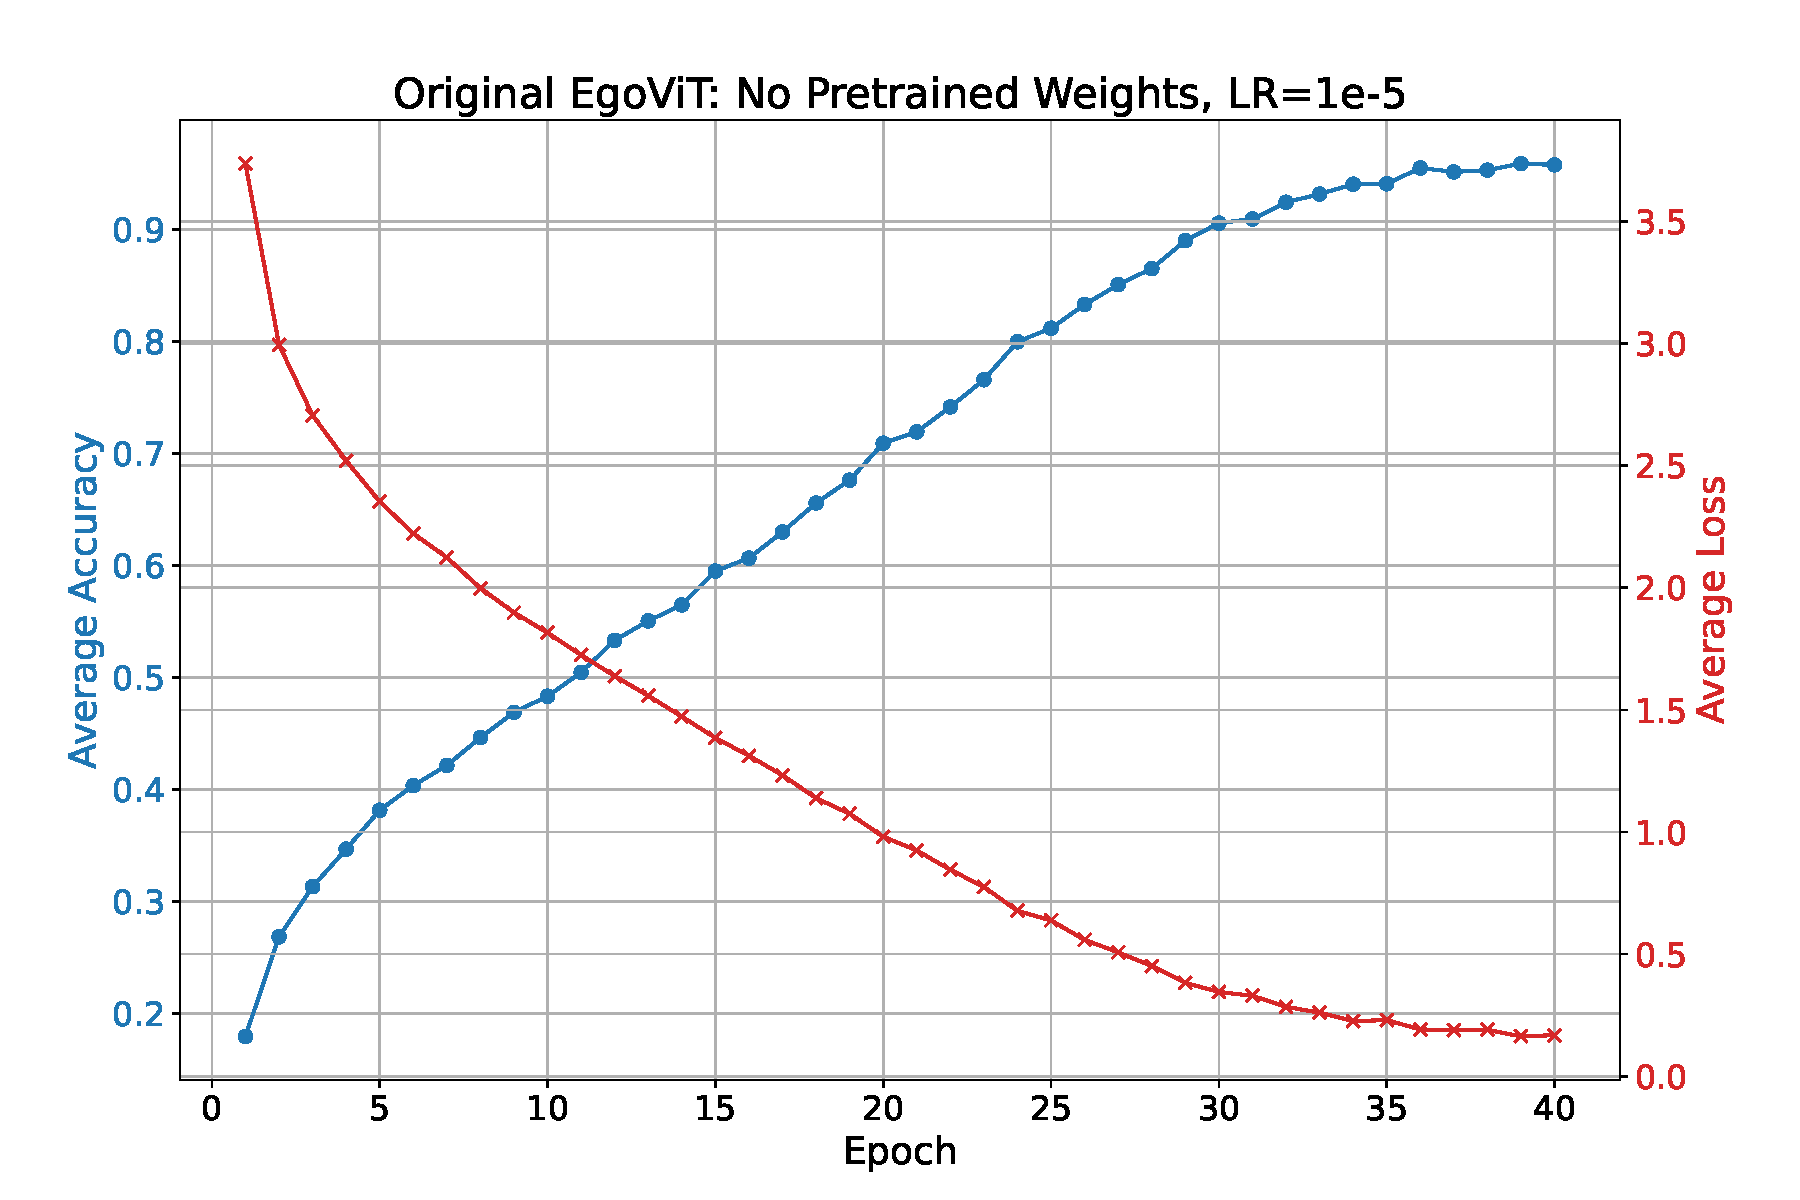
\includegraphics[width=0.9\linewidth]{assets/figure1.pdf}
            \caption{\parbox[t]{\linewidth}{Training accuracy and loss of the original EgoViT without pretrained weights.}}
            \label{fig:org_without_pre}
        \end{figure}
        \vfill
        \begin{figure}
            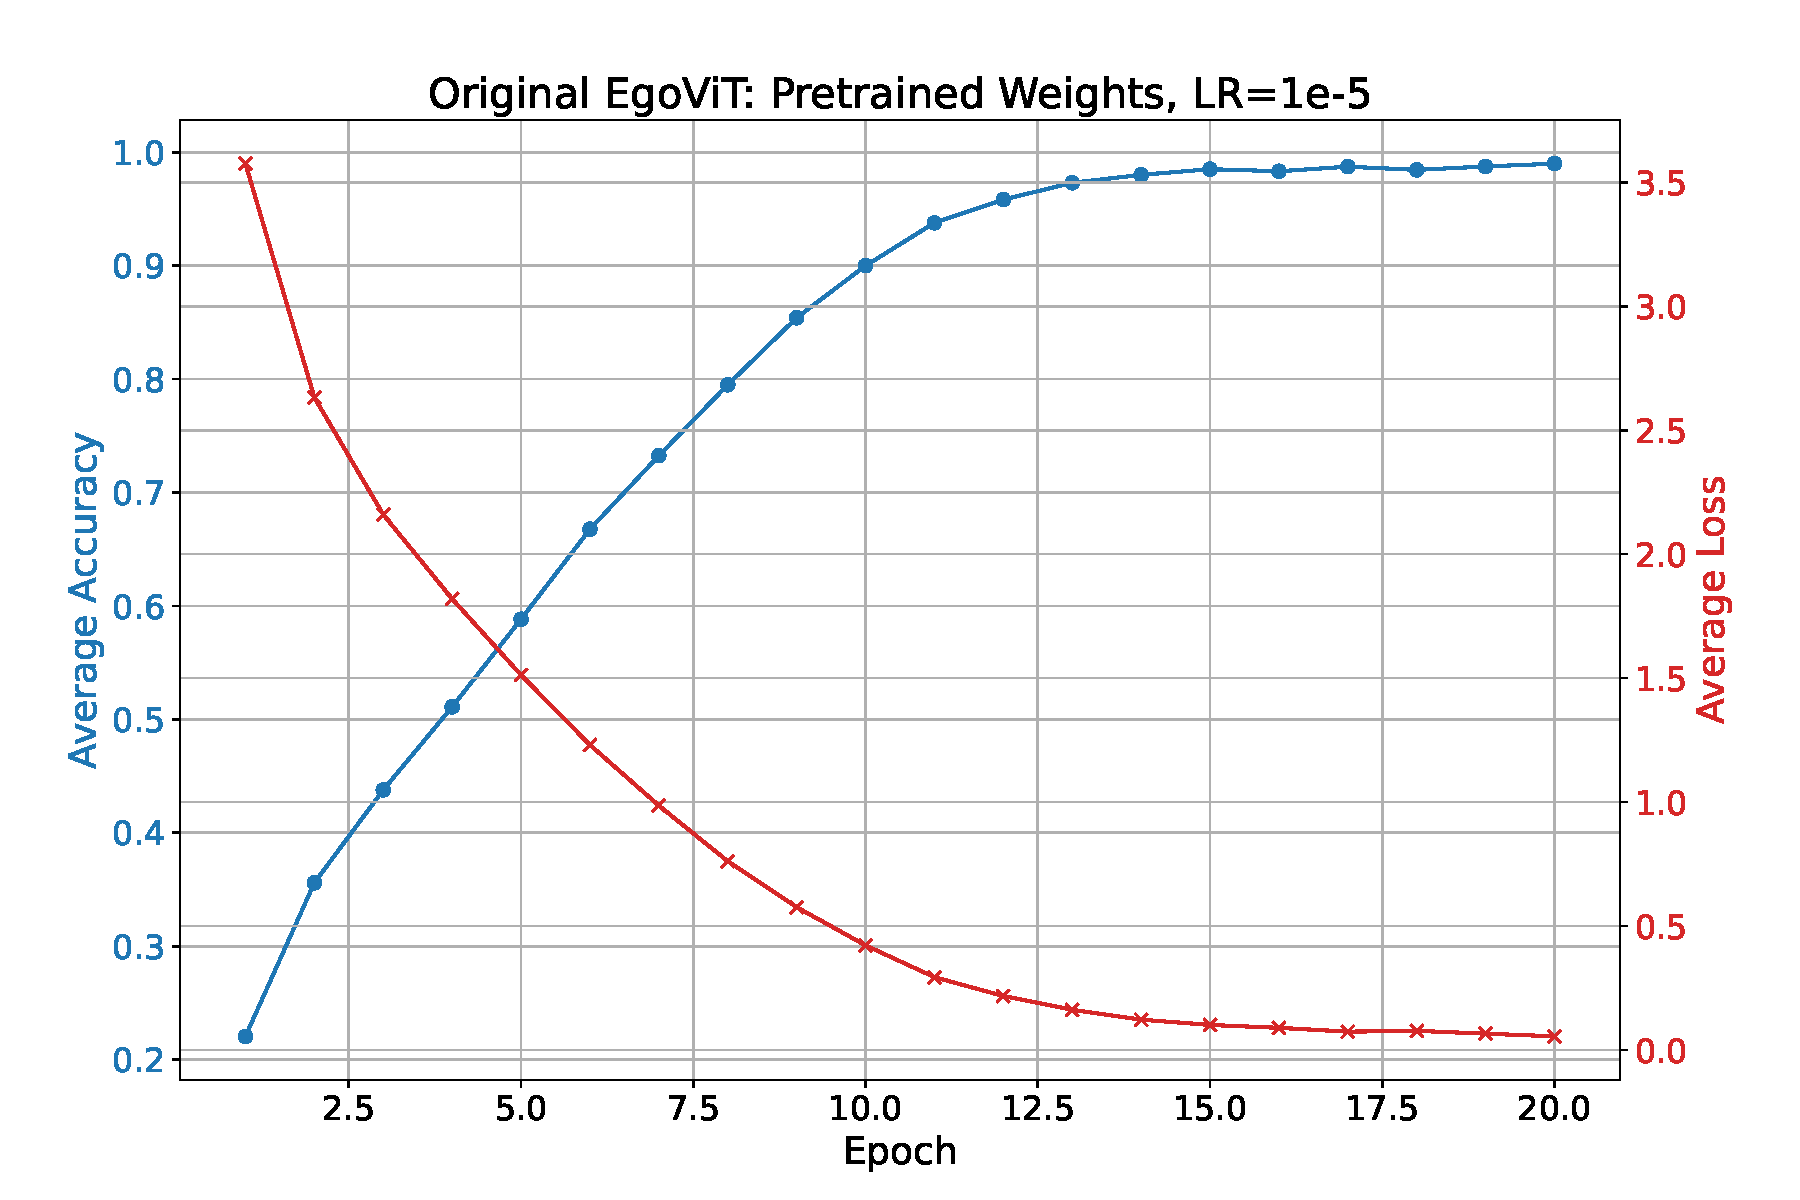
\includegraphics[width=0.9\linewidth]{assets/figure3.pdf}
            \caption{\parbox[t]{\linewidth}{Training accuracy and loss of the original EgoViT with pretrained weights.}}
            \label{fig:org_with_pre}
        \end{figure}
    \end{minipage}
	\hfill
	\begin{minipage}{0.45\textwidth}
		\begin{itemize}
			\item Both models reached similar training accuracy and loss.
			\item The model with pretrained weights converges faster.
		\end{itemize}
	\end{minipage}
\end{frame}

\begin{frame}{Training the Original EgoViT}
	\begin{minipage}{\textwidth}
		\begin{table}
			\centering
			{\textbf{Test Results of original EgoViT with HO Features}}
			\vspace{5mm}
			\resizebox{\linewidth}{!}{
			\begin{tabular}{lccc}
			\hline\hline
			Experiment ID & Top-1 Acc.(\%) & Top-5 Acc.(\%) & Mean Class Acc.(\%) \\
			\hline
			Orig\_HO\_no\_pretrain       & 51.5 & 78.5 & 38.8 \\
			Orig\_HO                     & 51.7 & 75.2 & 40.6 \\
			\hline\hline
			\end{tabular}
			}
			\label{tab:original-egovit}
		\end{table}
	\end{minipage}
	% \vfill
	\begin{minipage}{\textwidth}
		\textbf{Analysis:}
		\begin{itemize}
			\item The model with pretrained weights has higher top-1 and mean class accuracy
			\item Pretrained weights reduce the training time significantly
		\end{itemize}
	\end{minipage}
\end{frame}

% \begin{frame}{Dataset Modifications}
% 	\begin{minipage}{0.5\textwidth}
% 	\begin{itemize}
% 		\item Random gaze-box for videos without gaze information.
% 		\item Generate random hand and object features for videos lacking these elements.
% 	\end{itemize}
% 	\end{minipage}
% 	\hfill
% 	\begin{minipage}{0.45\textwidth}
% 	\begin{figure}
% 		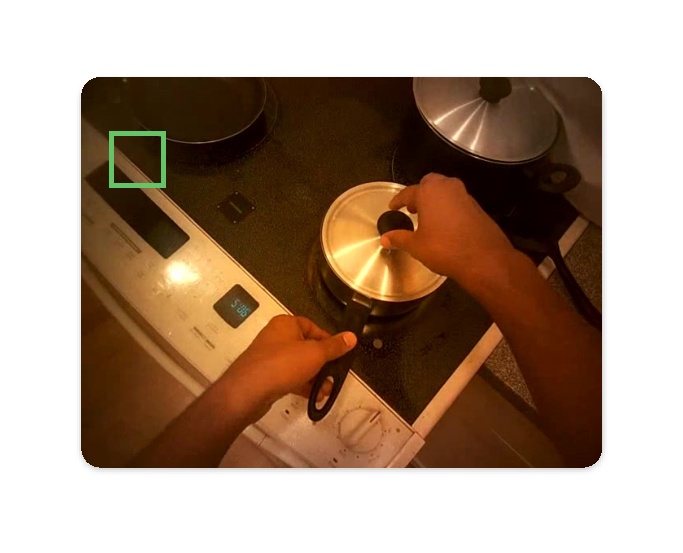
\includegraphics[width=1\linewidth]{assets/random_box}
% 		\caption{An example frame modified with random gaze-box (green).}
% 		\label{fig:random box}
% 	\end{figure}
% 	\end{minipage}
% \end{frame}


\begin{frame}{Training the Gaze Enhanced EgoViT}
	\begin{minipage}{\textwidth}
		\begin{table}
			\centering
			\textbf{Test Results of Original EgoViT with HO Features}
			\vspace{3mm}
			\begin{tabular}{lccc}
			\hline\hline
			Experiment ID & Top-1 Acc. & Top-5 Acc. & Mean Class Acc. \\
			\hline
			Orig\_HO        & 51.7 & 75.2 & 40.6 \\
			Enh\_GHO     & 51.4 & 76.7 & 40.0 \\
			Enh\_G       & 48.9 & 75.1 & 37.7 \\
			\hline\hline
			\end{tabular}
			\label{tab:Results_table2}
		\end{table}
	\end{minipage}
	\vfill
	\begin{minipage}{\textwidth}
		\textbf{Analysis:} 
		\begin{itemize}
			\item Enh\_GHO: slightly lower top-1 and mean class accuracy than Orig\_HO.
			\item Enh\_G: Lowest accuracy among the three models.
			\item The gaze features need further improvement.
		\end{itemize}
	\end{minipage}
\end{frame}

\begin{frame}{Training the Gaze Enhanced EgoViT}
	\textbf{Improve the quantity of the gaze data} 
	\begin{itemize}
		% \item Improve the quantity of the gaze data
		\item Gaze version 1 (GHO \& G): Uses only fixation gaze tracking data.
		\item Gaze version 2 (GHO\_v2 \& G\_v2): Uses both fixation and saccade gaze tracking data.
		\item Gaze version 2 has fewer random gaze features, enhancing the overall data quality.
	\end{itemize}
\end{frame}

\begin{frame}{Training the Gaze Enhanced EgoViT}
	\begin{minipage}{\textwidth}
	\begin{table}
		% \centering
		\textbf{Test Results on Gaze Version 1 and Gaze Version 2}
		\vspace{5mm}
		\resizebox{\linewidth}{!}{
		\begin{tabular}{lccc}
		\hline\hline
		Experiment ID & Top-1 Acc.(\%)& Top-5 Acc.(\%)& Mean Class Acc.(\%) \\
		\hline
		Enh\_GHO     & 51.4 & 76.7 & 40.0 \\
		Enh\_G       & 48.9 & 75.1 & 37.7 \\
		Enh\_GHO\_v2 & 52.0 & 76.3 & 38.7 \\
		Enh\_G\_v2   & 50.0 & 76.2 & 38.0 \\
		\hline\hline
		\end{tabular}}
		\label{tab:Results_table3}
		\end{table}
	\end{minipage}
	\begin{minipage}{\textwidth}
		\textbf{Analysis:}
		\begin{itemize}
			\item Enh\_G\_v2 shows significant improvement in all three metrics.
			\item The quality of gaze features is important for action recognition.
		\end{itemize}
	\end{minipage}
\end{frame}

% \begin{frame}{Training the Gaze Enhanced EgoViT}
% 	\begin{minipage}{\textwidth}
% 		\begin{figure}
% 			\centering
% 			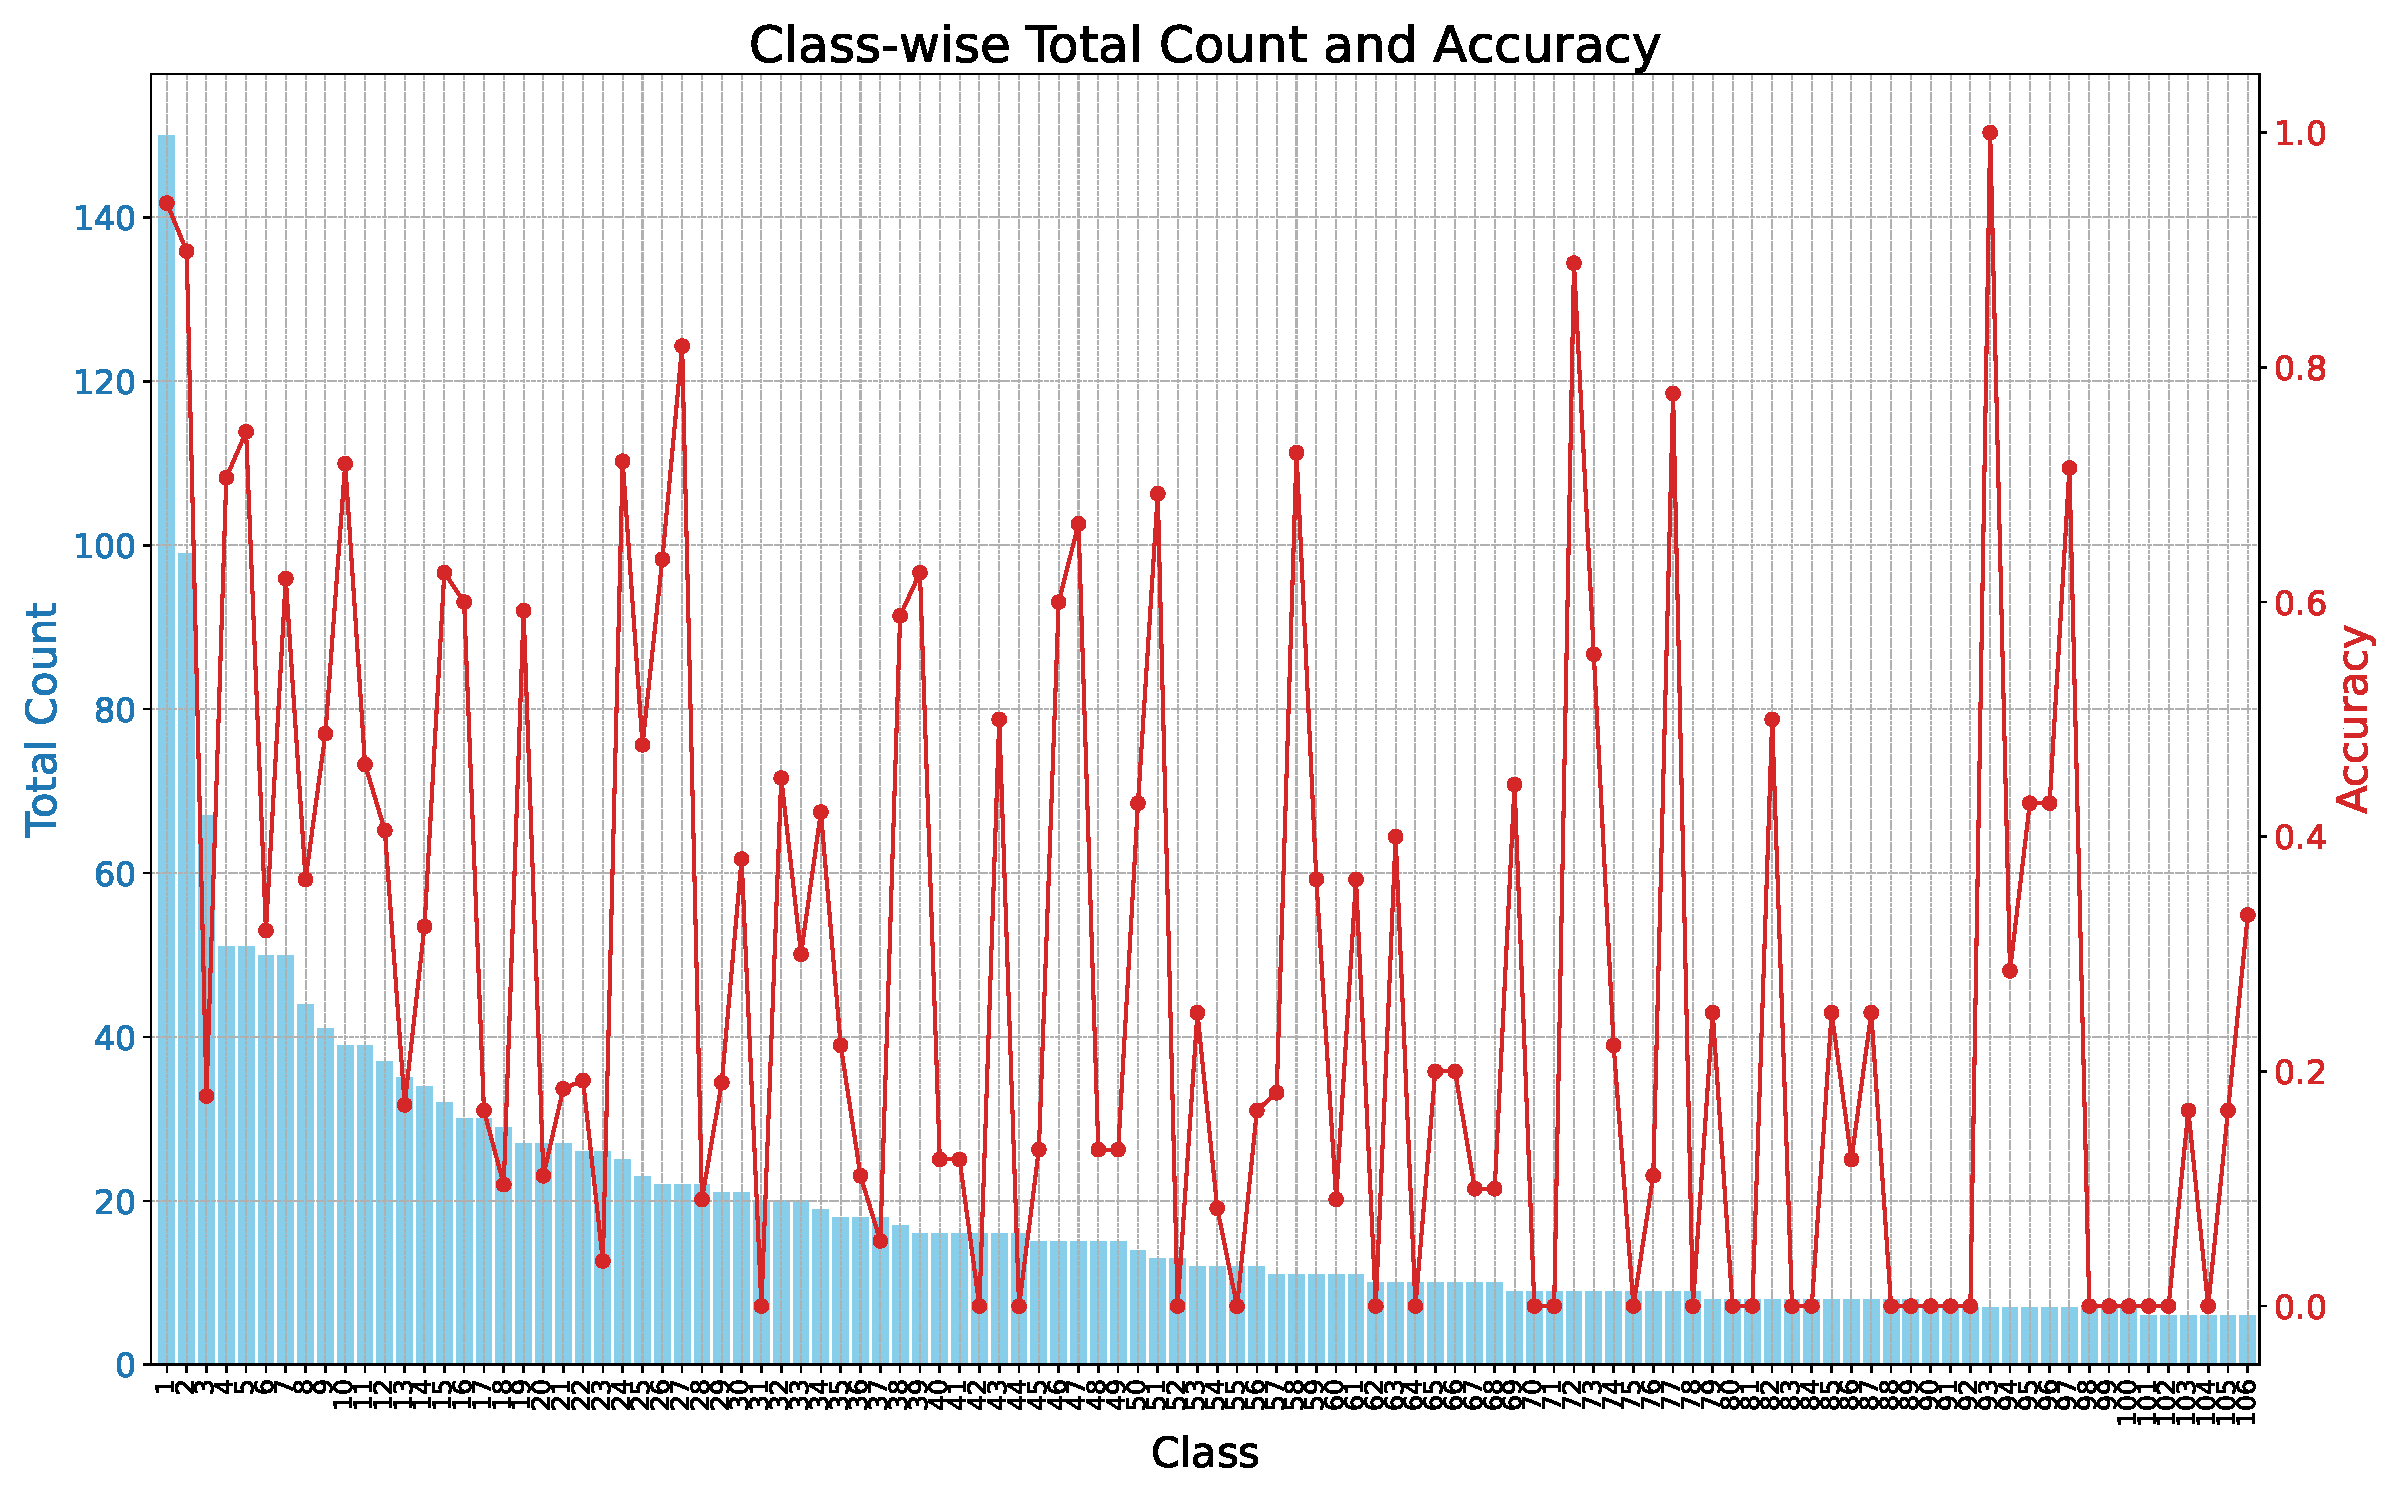
\includegraphics[width=0.8\linewidth]{assets/2in1.pdf}
% 			\caption{dd}
% 			\label{fig:class-wise total count}
% 		\end{figure}
% 	\end{minipage}
% 	\vfill
% 	\begin{minipage}{\textwidth}
% 		\begin{itemize}
% 			\item Dataset is imbalanced and many classes have zero accuracy
% 			\item d
% 		\end{itemize}
% 	\end{minipage}
% \end{frame}

\begin{frame}{Training EgoViT Variants}
	\begin{minipage}{0.5\textwidth}
		\begin{figure}
			\centering
			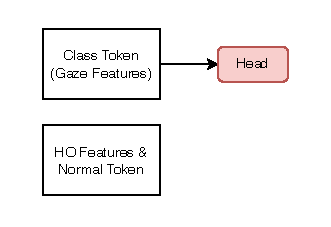
\includegraphics[width=\linewidth]{assets/version2.pdf}
			\caption{Enhanced EgoViT Version 2}
			\label{fig:version2}
		\end{figure}
		\begin{figure}
			\centering
			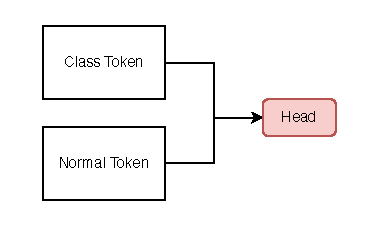
\includegraphics[width=\linewidth]{assets/version3.pdf}
			\caption{EgoViT Version 3}
			\label{fig:version3}
		\end{figure}
	\end{minipage}
	\hfill
	\begin{minipage}{0.45\textwidth}
		\begin{itemize}
			\item Enh\_v2\_GHO\_: Uses only gaze features for classification.
			\vspace{25mm}
			
			\item Orig\_v3, Enh\_v3: Use class token and normal token for classification.
		\end{itemize}
	\end{minipage}
\end{frame}

% \begin{frame}{d}
% 	\begin{minipage}{\textwidth}
% 		\begin{figure}
% 			\centering
% 			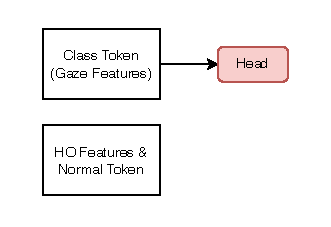
\includegraphics[width=0.8\linewidth]{assets/version2.pdf}
% 			\caption{dd}
% 			\label{fig:version2}
% 		\end{figure}
% 		\begin{itemize}
% 			\item Enh\_v2\_GHO\_: Using only gaze features to classify
% 			\item Orig\_v3, Enh\_v3: Using class token and normal token to classify

% 		\end{itemize}
% 	\end{minipage}
% \end{frame}

\begin{frame}{Training EgoViT Variants}
	\begin{minipage}{\textwidth}
		\begin{table}
			\centering
			\textbf{Test Results on EgoViT Variants}
			\resizebox{\linewidth}{!}{
			\begin{tabular}{lccc}
			\hline\hline
			Training Method & Top-1 Acc.(\%)& Top-5 Acc.(\%)& Mean Class Acc.(\%) \\
			\hline
			Enh\_GHO\_v2 & 52.0 & 76.3 & 38.7 \\
			Enh\_v2\_GHO\_v2 & 50.4 & 75.8 & 38.3 \\
			Enh\_v3\_GHO\_v2 & 51.2 & 77.9 & 39.2 \\
			\hline
			Orig\_HO        & 51.7 & 75.2 & 40.6 \\
			Orig\_v3\_HO & 51.1 & 77.4 & 40.5 \\
			\hline
			Enh\_G\_v2   & 50.0 & 76.2 & 38.0 \\
			Enh\_v3\_G\_v2   & 50.8 & 75.9 & 37.8 \\
			\hline\hline
			\end{tabular}}
			\label{tab:Results_table4}
		\end{table}
	\end{minipage}
	\begin{minipage}{\textwidth}
		\textbf{Analysis:}
		\begin{itemize}
			% \item The model with class token and normal token: higher accuracy
			% \item Enh\_v2 shows lower performance
			\item Merged GHO features are more effective
			% \item Enh\_v3 and Orig\_v3 improve only top-5 accuracy
			\item Class token has enough information for classification
			% \item Information in the class token and normal token are already exchanged in 3D Shifted Window Self-Attention
		\end{itemize}
		% \textbf{Possible Reason:} Information in the class token and normal token is already exchanged in 3D Shifted Window Self-Attention.
	\end{minipage}
\end{frame}

\begin{frame}{Distribution of Dataset}
	\begin{minipage}{\textwidth}
		\begin{figure}
			\centering
			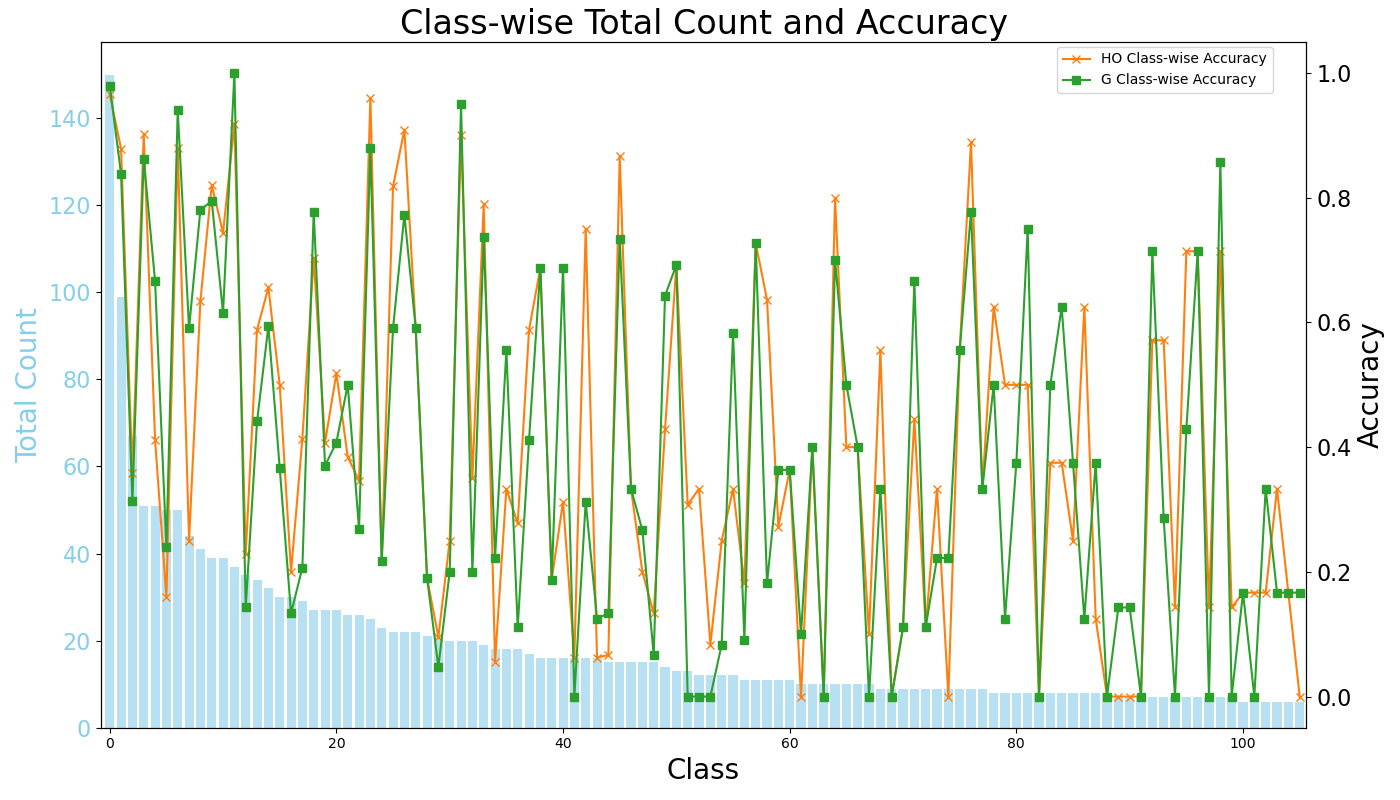
\includegraphics[width=0.85\linewidth]{assets/3in1.png}
			\caption{Visualization of the dataset and model predictions.}
			\label{fig:3in1}
		\end{figure}
		\vfill
		\begin{minipage}{\textwidth}
			\begin{itemize}
				\item The dataset is imbalanced, leading to overfitting on the majority class.
				\item The model with gaze features performs poorly in predicting movement actions.
			\end{itemize}
		\end{minipage}
	\end{minipage}
\end{frame}

\section[Conclusion and Future Works]{Conclusion and Future Works}
% \begin{frame}{Current Progress}
% 	\textbf{Current progress:}
% 	\begin{itemize}
% 		\item Implementing the model code
% 		\item Began training the model on a 8299 videos dataset
% 	\end{itemize}
% 	\textbf{Result:}
% 	\begin{itemize}
% 		\item Model size: 277M parameters, EgoViT-SwinB: 88M
% 		\item Low training accuracy at 7\%, EgoViT-SwinB: 69.72\%
% 	\end{itemize}
% \end{frame}

\begin{frame}{Future Works}
	\textbf{Conclusion:}
	\begin{itemize}
		\item Incorporating additional gaze features could enhance the model's performance.
		\item The quality of the gaze features is crucial for improving the accuracy of action recognition.
	\end{itemize}
	\vspace{5mm}
	\textbf{Future Works:}
	\begin{itemize}
	\item Investigate the impact of gaze region size.
	\item Utilize pretrained networks, such as an Autoencoders, to generate gaze features.
	\end{itemize}
\end{frame}
% \begin{frame}[fragile]{Timetable}
% 	\begin{figure}
% 		\centering
% 		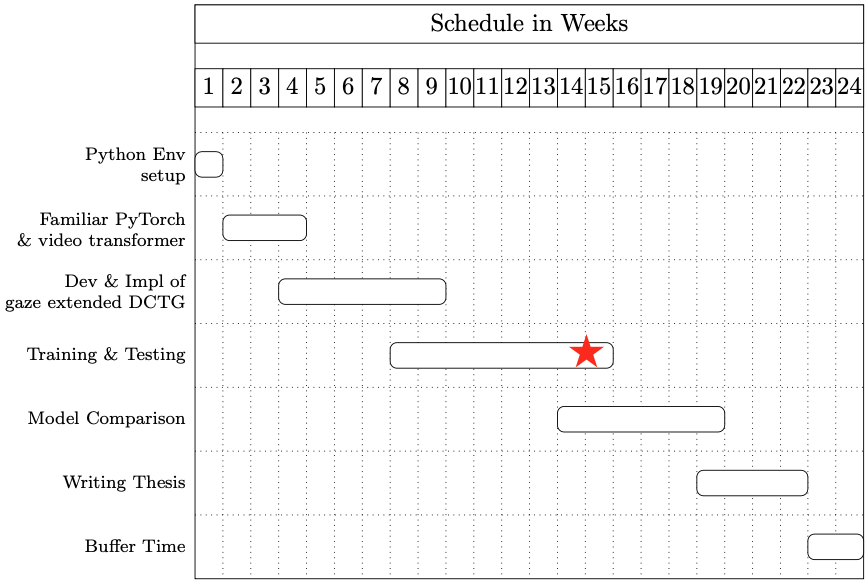
\includegraphics[width=0.8\linewidth]{assets/timetable} 
% 		%\caption{Timetable}
% 		\label{fig:timetable}
% 	\end{figure}
% \end{frame}
\begin{frame}
	\centering
	\Huge
	% \emph{Thank You!}
	\textbf{Thank You!}
\end{frame}
\begin{frame}[allowframebreaks]{References}
\bibliographystyle{abbrvnat}
{\scriptsize
  \bibliography{references}
}
\end{frame}

%\begin{frame}[standout]
%Thank you!
%\end{frame}

\end{document}


